\section{Theoretisch Kader} \label{sec:TheoretischKader}

In dit hoofdstuk wordt de theorie achter de motordrive en de testprotocollen uitgelegd.

\subsection{Motor Testen}

Voorheen werden de spindels die getest werden op de testkast alleen bekeken of deze draaiden en of deze niet te veel trilden. Hierbij werden geen meetgegevens gekwantifiseerd, waardoor er eigenlijk niet veel gezegd kan worden over de staat van de motor met duidelijke meetgegevens. Het zou voor de klant, maar ook voor Voortman, toegevoegde waarde hebben om meetgegevens van de motor te kwantifiseren en deze ook statistisch te beoordelen in een testrapport. Voortman kan op deze manier bewijzen dat de spindel weer correct werkt en in wat voor staat de spindel zich momenteel bevindt.

\subsubsection{Fast Fourier Transformation}

Veel motortesten maken gebruik van een Fourier transformatie om op deze manier iets te kunnen zeggen over het frequentiedomein van de meetgegevens. De Discrete Fourier Transform (\gls{DFT}) converteert een eindige reeks van op een gelijke afstand geplaatste reeks van samples van dezelfde lengte van de discrete-time Fourier transformatie (\gls{DTFT}), wat een frequentiefunctie met complexe getallen is. De \gls{DFT} is een frequentiedomeinrepresentatie van de originele invoerreeks (figuur \ref{fig:FourierTransform}).

\begin{figure}[h]
	\centering
	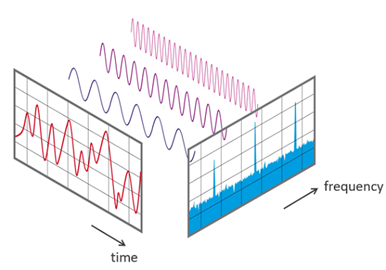
\includegraphics[width=300pt]{FourierTransform}
	\label{fig:FourierTransform}
	\caption{Fourier Transformatie \cite{web:FFT}}
\end{figure}

\newpage

De formule voor de \gls{DFT} is als volgt:

\begin{equation}
	X_k = \sum_{n=0}^{N-1}X_n e^{-i2\pi\frac{k}{N}n}
\end{equation}

Echter kan deze formule erg intensief zijn bij een hoog aantal samples daarom is het beter om een \gls{FFT} te gebruiken zoals het Radix-2 algoritme die het aantal berekeningen aanzienlijk verminderd \cite{web:FFT}:

\begin{equation}
	X_k = {\sum_{m=0}^{\frac{N}{2}-1}X_{2m}e^{-\frac{2\pi i}{N}(2m)k}} + {\sum_{m=0}^{\frac{N}{2}-1}X_{2m+1}e^{-\frac{2\pi i}{N}(2m+1)k}}
\end{equation}

Het idee achter het Radix-2 algoritme is dat eerst alle even getallen berekend worden en hierna de oneven getallen waarna de resultaten gecombineerd worden. Vervolgens kan dit recursief worden berekend. De enige eis hiervan is dat de sample set grootte een macht van 2 moet zijn \cite{web:Radix-2FFT}.

\subsubsection{Lager schade detectie}

De meeste gevallen van motorstoringen komen door slijtage of schade aan de lagers. Lagerschade kan worden gedetecteerd onder andere door het meten van de trillingen van de motor of spindel. Hierbij kan men vier frequentie pieken berekenen in de \gls{FFT} van de trillingen van de spindel waardoor de oorzaak van de schade of de staat van de lager kan worden bepaaldt. Lager schade vormt zich in vier fasen, in de een na laatste fase zullen de berekende pieken zich vormen. Het vervangen van de lager is op dat moment noodzakelijk aangezien de lager het uiteindelijk zal begeven in de laatste fase \cite{web:BearingFault}. Voor meer informatie over deze fasen zie bijlage \ref{sec:LiteratuurOnderzoek} hoofdstuk 6.


\begin{figure}[h]
	\centering
	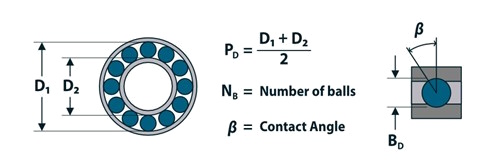
\includegraphics[width=350pt]{LagerSchade}
	\label{fig:LagerSchade}
	\caption{Lager schade herkennen door trillingen \cite{web:BearingFault}}
\end{figure}

\begin{enumerate}
	\item \textbf{Balls Pass Frequency Outer Race (\gls{BPFO})} Deze frequentie komt overeen met het aantal kogels dat door een bepaald punt van de buitenring gaat bij elke volledige draai.
	
	\begin{equation}
		BPFO = RPM\frac{N_b}{2}(1-\frac{B_D}{P_D}\cos\cos\beta)
	\end{equation}
	\newpage
	
	\item \textbf{Ball Pass Frequency Inner Race (\gls{BPFI})} Deze frequentie staat gelijk aan de binnenringstoringsfrequentie. Deze frequentie ontstaat doordat de kogels of rollers langs een bepaald punt komen bij elke rotatie.
	
	\begin{equation}
		BPFI = RPM\frac{N_b}{2}(1-\frac{B_D}{P_D}\cos \cos \beta)
	\end{equation}
	
	\item \textbf{Ball Spin Frequency (\gls{BSF})} Deze frequentie komt overeen met het aantal omwentelingen dat een lager kogel of rol maakt elke keer wanneer de as een volledige draai heeft gemaakt.
	
	\begin{equation}
		BSF = RPM\frac{P_D}{B_D}[1-(\frac{B_D}{P_D} \cos \cos \beta)^2]
	\end{equation}
	
	\item \textbf{Fundamental Train Frequency (\gls{FTF})} Deze frequentie komt overeen met het aantal omwentelingen die de lager kooi maakt bij elke volledige draai.
	
	\begin{equation}
		FTF=RPM\frac{1}{2}(1-\frac{B_D}{P_D} \cos \cos \beta)
	\end{equation}
\end{enumerate}

In figuur \ref{fig:LagerStage3} is een voorbeeld te zien hoe de berekende pieken te zien zouden kunnen zijn wanneer een lager in stage 3 is van zijn slijtage.

\begin{figure}[h]
	\centering
	
	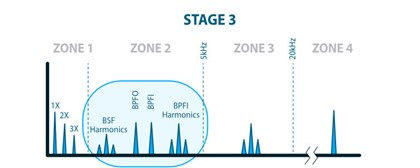
\includegraphics[width=400pt]{LagerStage3}
	
	\label{fig:LagerStage3}
	\caption{Berekende frequentie pieken in een \gls{FFT} van de trillingen \cite{web:BearingFault}}
\end{figure}

\newpage

\subsubsection{Rotor Excentriciteit}

Excentriciteit in de rotor zorgt ongeveer voor 12\% tot 16\% van alle motor storingen \cite{MotorExcenttriciteit}. Er zijn bij rotor excentriciteit twee smaken:

\begin{enumerate}
	\item \textbf{Dynamische excentriciteit} hierbij veranderd de afstand tussen de stator en de rotor constant waardoor er onbalans en trillingen kunnen ontstaan. Oorzaken hiervan kunnen zijn versleten lagers, mechanische speling of een kromme rotorstang.
	
	\item \textbf{Statische excentriciteit} hierbij is de rotor niet in het midden geplaatst van de stator. De afstand tussen de rotor en stator is hierbij constant. Statische excentriciteit zal zorgen voor ongelijke magnetische krachten wat weer zal resulteren in extra energieverbruik en meer slijtage in de lagers.
\end{enumerate}

